\documentclass[1p]{elsarticle_modified}
%\bibliographystyle{elsarticle-num}

%\usepackage[colorlinks]{hyperref}
%\usepackage{abbrmath_seonhwa} %\Abb, \Ascr, \Acal ,\Abf, \Afrak
\usepackage{amsfonts}
\usepackage{amssymb}
\usepackage{amsmath}
\usepackage{amsthm}
\usepackage{scalefnt}
\usepackage{amsbsy}
\usepackage{kotex}
\usepackage{caption}
\usepackage{subfig}
\usepackage{color}
\usepackage{graphicx}
\usepackage{xcolor} %% white, black, red, green, blue, cyan, magenta, yellow
\usepackage{float}
\usepackage{setspace}
\usepackage{hyperref}

\usepackage{tikz}
\usetikzlibrary{arrows}

\usepackage{multirow}
\usepackage{array} % fixed length table
\usepackage{hhline}

%%%%%%%%%%%%%%%%%%%%%
\makeatletter
\renewcommand*\env@matrix[1][\arraystretch]{%
	\edef\arraystretch{#1}%
	\hskip -\arraycolsep
	\let\@ifnextchar\new@ifnextchar
	\array{*\c@MaxMatrixCols c}}
\makeatother %https://tex.stackexchange.com/questions/14071/how-can-i-increase-the-line-spacing-in-a-matrix
%%%%%%%%%%%%%%%

\usepackage[normalem]{ulem}

\newcommand{\msout}[1]{\ifmmode\text{\sout{\ensuremath{#1}}}\else\sout{#1}\fi}
%SOURCE: \msout is \stkout macro in https://tex.stackexchange.com/questions/20609/strikeout-in-math-mode

\newcommand{\cancel}[1]{
	\ifmmode
	{\color{red}\msout{#1}}
	\else
	{\color{red}\sout{#1}}
	\fi
}

\newcommand{\add}[1]{
	{\color{blue}\uwave{#1}}
}

\newcommand{\replace}[2]{
	\ifmmode
	{\color{red}\msout{#1}}{\color{blue}\uwave{#2}}
	\else
	{\color{red}\sout{#1}}{\color{blue}\uwave{#2}}
	\fi
}

\newcommand{\Sol}{\mathcal{S}} %segment
\newcommand{\D}{D} %diagram
\newcommand{\A}{\mathcal{A}} %arc


%%%%%%%%%%%%%%%%%%%%%%%%%%%%%5 test

\def\sl{\operatorname{\textup{SL}}(2,\Cbb)}
\def\psl{\operatorname{\textup{PSL}}(2,\Cbb)}
\def\quan{\mkern 1mu \triangleright \mkern 1mu}

\theoremstyle{definition}
\newtheorem{thm}{Theorem}[section]
\newtheorem{prop}[thm]{Proposition}
\newtheorem{lem}[thm]{Lemma}
\newtheorem{ques}[thm]{Question}
\newtheorem{cor}[thm]{Corollary}
\newtheorem{defn}[thm]{Definition}
\newtheorem{exam}[thm]{Example}
\newtheorem{rmk}[thm]{Remark}
\newtheorem{alg}[thm]{Algorithm}

\newcommand{\I}{\sqrt{-1}}
\begin{document}

%\begin{frontmatter}
%
%\title{Boundary parabolic representations of knots up to 8 crossings}
%
%%% Group authors per affiliation:
%\author{Yunhi Cho} 
%\address{Department of Mathematics, University of Seoul, Seoul, Korea}
%\ead{yhcho@uos.ac.kr}
%
%
%\author{Seonhwa Kim} %\fnref{s_kim}}
%\address{Center for Geometry and Physics, Institute for Basic Science, Pohang, 37673, Korea}
%\ead{ryeona17@ibs.re.kr}
%
%\author{Hyuk Kim}
%\address{Department of Mathematical Sciences, Seoul National University, Seoul 08826, Korea}
%\ead{hyukkim@snu.ac.kr}
%
%\author{Seokbeom Yoon}
%\address{Department of Mathematical Sciences, Seoul National University, Seoul, 08826,  Korea}
%\ead{sbyoon15@snu.ac.kr}
%
%\begin{abstract}
%We find all boundary parabolic representation of knots up to 8 crossings.
%
%\end{abstract}
%\begin{keyword}
%    \MSC[2010] 57M25 
%\end{keyword}
%
%\end{frontmatter}

%\linenumbers
%\tableofcontents
%
\newcommand\colored[1]{\textcolor{white}{\rule[-0.35ex]{0.8em}{1.4ex}}\kern-0.8em\color{red} #1}%
%\newcommand\colored[1]{\textcolor{white}{ #1}\kern-2.17ex	\textcolor{white}{ #1}\kern-1.81ex	\textcolor{white}{ #1}\kern-2.15ex\color{red}#1	}

{\Large $\underline{11n_{23}~(K11n_{23})}$}

\setlength{\tabcolsep}{10pt}
\renewcommand{\arraystretch}{1.6}
\vspace{1cm}\begin{tabular}{m{100pt}>{\centering\arraybackslash}m{274pt}}
\multirow{5}{120pt}{
	\centering
	\includegraphics[width=112pt]{../../../GIT/diagram.site/Diagrams/png/639_11n_23.png}\\
\ \ \ A knot diagram\footnotemark}&
\allowdisplaybreaks
\textbf{Linearized knot diagam} \\
\cline{2-2}
 &
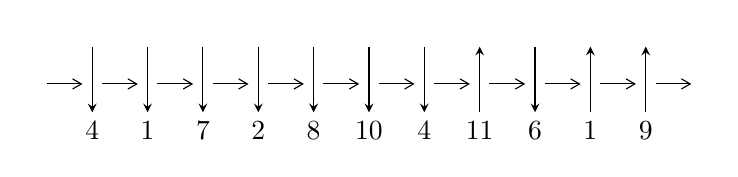
\begin{tikzpicture}[x=20pt, y=17pt]
	% nodes
	\node (C0) at (0, 0) {};
	\node (C1) at (1, 0) {};
	\node (C1U) at (1, +1) {};
	\node (C1D) at (1, -1) {4};

	\node (C2) at (2, 0) {};
	\node (C2U) at (2, +1) {};
	\node (C2D) at (2, -1) {1};

	\node (C3) at (3, 0) {};
	\node (C3U) at (3, +1) {};
	\node (C3D) at (3, -1) {7};

	\node (C4) at (4, 0) {};
	\node (C4U) at (4, +1) {};
	\node (C4D) at (4, -1) {2};

	\node (C5) at (5, 0) {};
	\node (C5U) at (5, +1) {};
	\node (C5D) at (5, -1) {8};

	\node (C6) at (6, 0) {};
	\node (C6U) at (6, +1) {};
	\node (C6D) at (6, -1) {10};

	\node (C7) at (7, 0) {};
	\node (C7U) at (7, +1) {};
	\node (C7D) at (7, -1) {4};

	\node (C8) at (8, 0) {};
	\node (C8U) at (8, +1) {};
	\node (C8D) at (8, -1) {11};

	\node (C9) at (9, 0) {};
	\node (C9U) at (9, +1) {};
	\node (C9D) at (9, -1) {6};

	\node (C10) at (10, 0) {};
	\node (C10U) at (10, +1) {};
	\node (C10D) at (10, -1) {1};

	\node (C11) at (11, 0) {};
	\node (C11U) at (11, +1) {};
	\node (C11D) at (11, -1) {9};
	\node (C12) at (12, 0) {};

	% arrows
	\draw[->,>={angle 60}]
	(C0) edge (C1) (C1) edge (C2) (C2) edge (C3) (C3) edge (C4) (C4) edge (C5) (C5) edge (C6) (C6) edge (C7) (C7) edge (C8) (C8) edge (C9) (C9) edge (C10) (C10) edge (C11) (C11) edge (C12) ;	\draw[->,>=stealth]
	(C1U) edge (C1D) (C2U) edge (C2D) (C3U) edge (C3D) (C4U) edge (C4D) (C5U) edge (C5D) (C6U) edge (C6D) (C7U) edge (C7D) (C8D) edge (C8U) (C9U) edge (C9D) (C10D) edge (C10U) (C11D) edge (C11U) ;
	\end{tikzpicture} \\
\hhline{~~} \\& 
\textbf{Solving Sequence} \\ \cline{2-2} 
 &
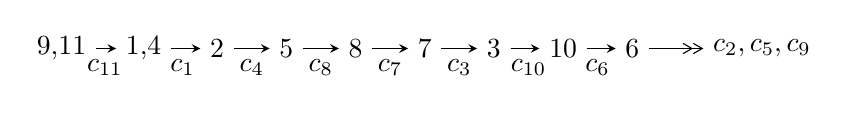
\begin{tikzpicture}[x=25pt, y=7pt]
	% node
	\node (A0) at (-1/8, 0) {9,11};
	\node (A1) at (17/16, 0) {1,4};
	\node (A2) at (17/8, 0) {2};
	\node (A3) at (25/8, 0) {5};
	\node (A4) at (33/8, 0) {8};
	\node (A5) at (41/8, 0) {7};
	\node (A6) at (49/8, 0) {3};
	\node (A7) at (57/8, 0) {10};
	\node (A8) at (65/8, 0) {6};
	\node (C1) at (1/2, -1) {$c_{11}$};
	\node (C2) at (13/8, -1) {$c_{1}$};
	\node (C3) at (21/8, -1) {$c_{4}$};
	\node (C4) at (29/8, -1) {$c_{8}$};
	\node (C5) at (37/8, -1) {$c_{7}$};
	\node (C6) at (45/8, -1) {$c_{3}$};
	\node (C7) at (53/8, -1) {$c_{10}$};
	\node (C8) at (61/8, -1) {$c_{6}$};
	\node (A9) at (10, 0) {$c_{2},c_{5},c_{9}$};

	% edge
	\draw[->,>=stealth]	
	(A0) edge (A1) (A1) edge (A2) (A2) edge (A3) (A3) edge (A4) (A4) edge (A5) (A5) edge (A6) (A6) edge (A7) (A7) edge (A8) ;
	\draw[->>,>={angle 60}]	
	(A8) edge (A9);
\end{tikzpicture} \\ 

\end{tabular} \\

\footnotetext{
The image of knot diagram is generated by the software ``\textbf{Draw programme}" developed by Andrew Bartholomew(\url{http://www.layer8.co.uk/maths/draw/index.htm\#Running-draw}), where we modified some parts for our purpose(\url{https://github.com/CATsTAILs/LinksPainter}).
}\phantom \\ \newline 
\centering \textbf{Ideals for irreducible components\footnotemark of $X_{\text{par}}$} 
 
\begin{align*}
I^u_{1}&=\langle 
-68646 u^{21}-209213 u^{20}+\cdots+105421 b-71719,\\
\phantom{I^u_{1}}&\phantom{= \langle  }-179395 u^{21}-675073 u^{20}+\cdots+210842 a-1064489,\;u^{22}+4 u^{21}+\cdots+8 u+1\rangle \\
I^u_{2}&=\langle 
- u^4- u^3+b+u,\;u^4+u^3+a- u,\;u^6+u^5- u^4-2 u^3+u+1\rangle \\
I^u_{3}&=\langle 
b+1,\;a^2- a-1,\;u-1\rangle \\
\\
\end{align*}
\raggedright * 3 irreducible components of $\dim_{\mathbb{C}}=0$, with total 30 representations.\\
\footnotetext{All coefficients of polynomials are rational numbers. But the coefficients are sometimes approximated in decimal forms when there is not enough margin.}
\newpage
\renewcommand{\arraystretch}{1}
\centering \section*{I. $I^u_{1}= \langle -6.86\times10^{4} u^{21}-2.09\times10^{5} u^{20}+\cdots+1.05\times10^{5} b-7.17\times10^{4},\;-1.79\times10^{5} u^{21}-6.75\times10^{5} u^{20}+\cdots+2.11\times10^{5} a-1.06\times10^{6},\;u^{22}+4 u^{21}+\cdots+8 u+1 \rangle$}
\flushleft \textbf{(i) Arc colorings}\\
\begin{tabular}{m{7pt} m{180pt} m{7pt} m{180pt} }
\flushright $a_{9}=$&$\begin{pmatrix}0\\u\end{pmatrix}$ \\
\flushright $a_{11}=$&$\begin{pmatrix}1\\0\end{pmatrix}$ \\
\flushright $a_{1}=$&$\begin{pmatrix}1\\- u^2\end{pmatrix}$ \\
\flushright $a_{4}=$&$\begin{pmatrix}0.850850 u^{21}+3.20180 u^{20}+\cdots+4.49725 u+5.04875\\0.651161 u^{21}+1.98455 u^{20}+\cdots+2.21543 u+0.680310\end{pmatrix}$ \\
\flushright $a_{2}=$&$\begin{pmatrix}0.315042 u^{21}+1.37186 u^{20}+\cdots+0.488432 u+3.18691\\0.182947 u^{21}+0.441795 u^{20}+\cdots-0.201113 u+0.0840297\end{pmatrix}$ \\
\flushright $a_{5}=$&$\begin{pmatrix}0.146826 u^{21}+1.01918 u^{20}+\cdots+1.95979 u+3.15823\\0.351163 u^{21}+0.794481 u^{20}+\cdots-1.67248 u+0.112710\end{pmatrix}$ \\
\flushright $a_{8}=$&$\begin{pmatrix}- u\\u\end{pmatrix}$ \\
\flushright $a_{7}=$&$\begin{pmatrix}-0.112710 u^{21}-0.0996765 u^{20}+\cdots-0.646560 u-2.57416\\0.431873 u^{21}+0.691897 u^{20}+\cdots+1.98362 u-0.146826\end{pmatrix}$ \\
\flushright $a_{3}=$&$\begin{pmatrix}0.688814 u^{21}+2.58804 u^{20}+\cdots+1.89815 u+3.21457\\-0.166694 u^{21}-0.538261 u^{20}+\cdots-2.05866 u-0.194885\end{pmatrix}$ \\
\flushright $a_{10}=$&$\begin{pmatrix}- u^2+1\\u^4\end{pmatrix}$ \\
\flushright $a_{6}=$&$\begin{pmatrix}-0.317366 u^{21}-1.15089 u^{20}+\cdots-1.03139 u-2.97993\\-0.180623 u^{21}-0.662766 u^{20}+\cdots+0.744069 u-0.291009\end{pmatrix}$\\ \flushright $a_{6}=$&$\begin{pmatrix}-0.317366 u^{21}-1.15089 u^{20}+\cdots-1.03139 u-2.97993\\-0.180623 u^{21}-0.662766 u^{20}+\cdots+0.744069 u-0.291009\end{pmatrix}$\\&\end{tabular}
\flushleft \textbf{(ii) Obstruction class $= -1$}\\~\\
\flushleft \textbf{(iii) Cusp Shapes $= \frac{98871}{105421} u^{21}+\frac{399034}{105421} u^{20}+\cdots+\frac{1542002}{105421} u-\frac{1060356}{105421}$}\\~\\
\newpage\renewcommand{\arraystretch}{1}
\flushleft \textbf{(iv) u-Polynomials at the component}\newline \\
\begin{tabular}{m{50pt}|m{274pt}}
Crossings & \hspace{64pt}u-Polynomials at each crossing \\
\hline $$\begin{aligned}c_{1},c_{4}\end{aligned}$$&$\begin{aligned}
&u^{22}-8 u^{21}+\cdots-10 u+1
\end{aligned}$\\
\hline $$\begin{aligned}c_{2}\end{aligned}$$&$\begin{aligned}
&u^{22}+36 u^{21}+\cdots+6 u+1
\end{aligned}$\\
\hline $$\begin{aligned}c_{3},c_{7}\end{aligned}$$&$\begin{aligned}
&u^{22}+2 u^{21}+\cdots+128 u^2+64
\end{aligned}$\\
\hline $$\begin{aligned}c_{5}\end{aligned}$$&$\begin{aligned}
&u^{22}-3 u^{21}+\cdots- u+1
\end{aligned}$\\
\hline $$\begin{aligned}c_{6},c_{9}\end{aligned}$$&$\begin{aligned}
&u^{22}+2 u^{21}+\cdots+28 u+4
\end{aligned}$\\
\hline $$\begin{aligned}c_{8},c_{11}\end{aligned}$$&$\begin{aligned}
&u^{22}+4 u^{21}+\cdots+8 u+1
\end{aligned}$\\
\hline $$\begin{aligned}c_{10}\end{aligned}$$&$\begin{aligned}
&u^{22}-8 u^{21}+\cdots-64 u+1
\end{aligned}$\\
\hline
\end{tabular}\\~\\
\newpage\renewcommand{\arraystretch}{1}
\flushleft \textbf{(v) Riley Polynomials at the component}\newline \\
\begin{tabular}{m{50pt}|m{274pt}}
Crossings & \hspace{64pt}Riley Polynomials at each crossing \\
\hline $$\begin{aligned}c_{1},c_{4}\end{aligned}$$&$\begin{aligned}
&y^{22}-36 y^{21}+\cdots-6 y+1
\end{aligned}$\\
\hline $$\begin{aligned}c_{2}\end{aligned}$$&$\begin{aligned}
&y^{22}-92 y^{21}+\cdots+3898 y+1
\end{aligned}$\\
\hline $$\begin{aligned}c_{3},c_{7}\end{aligned}$$&$\begin{aligned}
&y^{22}-42 y^{21}+\cdots+16384 y+4096
\end{aligned}$\\
\hline $$\begin{aligned}c_{5}\end{aligned}$$&$\begin{aligned}
&y^{22}-49 y^{21}+\cdots-17 y+1
\end{aligned}$\\
\hline $$\begin{aligned}c_{6},c_{9}\end{aligned}$$&$\begin{aligned}
&y^{22}-18 y^{21}+\cdots-264 y+16
\end{aligned}$\\
\hline $$\begin{aligned}c_{8},c_{11}\end{aligned}$$&$\begin{aligned}
&y^{22}-8 y^{21}+\cdots-64 y+1
\end{aligned}$\\
\hline $$\begin{aligned}c_{10}\end{aligned}$$&$\begin{aligned}
&y^{22}+16 y^{21}+\cdots-3112 y+1
\end{aligned}$\\
\hline
\end{tabular}\\~\\
\newpage\flushleft \textbf{(vi) Complex Volumes and Cusp Shapes}
$$\begin{array}{c|c|c}  
\text{Solutions to }I^u_{1}& \I (\text{vol} + \sqrt{-1}CS) & \text{Cusp shape}\\
 \hline 
\begin{aligned}
u &= \phantom{-}0.949302 + 0.242875 I \\
a &= \phantom{-}0.659054 + 0.118437 I \\
b &= -0.606013 - 0.510709 I\end{aligned}
 & \phantom{-}1.72824 + 0.76607 I & \phantom{-}3.12936 - 1.22783 I \\ \hline\begin{aligned}
u &= \phantom{-}0.949302 - 0.242875 I \\
a &= \phantom{-}0.659054 - 0.118437 I \\
b &= -0.606013 + 0.510709 I\end{aligned}
 & \phantom{-}1.72824 - 0.76607 I & \phantom{-}3.12936 + 1.22783 I \\ \hline\begin{aligned}
u &= \phantom{-}1.06873\phantom{ +0.000000I} \\
a &= \phantom{-}2.88944\phantom{ +0.000000I} \\
b &= -2.44319\phantom{ +0.000000I}\end{aligned}
 & \phantom{-}0.373053\phantom{ +0.000000I} & -36.4230\phantom{ +0.000000I} \\ \hline\begin{aligned}
u &= -0.611771 + 0.692060 I \\
a &= \phantom{-}0.790435 - 0.254867 I \\
b &= \phantom{-}0.122623 + 0.098224 I\end{aligned}
 & -2.04648 + 0.07308 I & -6.61841 + 0.32192 I \\ \hline\begin{aligned}
u &= -0.611771 - 0.692060 I \\
a &= \phantom{-}0.790435 + 0.254867 I \\
b &= \phantom{-}0.122623 - 0.098224 I\end{aligned}
 & -2.04648 - 0.07308 I & -6.61841 - 0.32192 I \\ \hline\begin{aligned}
u &= -0.831560\phantom{ +0.000000I} \\
a &= -0.842263\phantom{ +0.000000I} \\
b &= -0.991565\phantom{ +0.000000I}\end{aligned}
 & -7.60774\phantom{ +0.000000I} & -21.1720\phantom{ +0.000000I} \\ \hline\begin{aligned}
u &= -1.040460 + 0.605021 I \\
a &= \phantom{-}0.213779 - 0.135252 I \\
b &= -0.431084 + 0.709735 I\end{aligned}
 & -0.69505 - 5.13446 I & -2.61215 + 4.09914 I \\ \hline\begin{aligned}
u &= -1.040460 - 0.605021 I \\
a &= \phantom{-}0.213779 + 0.135252 I \\
b &= -0.431084 - 0.709735 I\end{aligned}
 & -0.69505 + 5.13446 I & -2.61215 - 4.09914 I \\ \hline\begin{aligned}
u &= -0.837414 + 0.879532 I \\
a &= -0.820247 + 0.387550 I \\
b &= \phantom{-}0.79848 - 1.81489 I\end{aligned}
 & -6.52288 - 1.21996 I & -10.21847 + 1.61822 I \\ \hline\begin{aligned}
u &= -0.837414 - 0.879532 I \\
a &= -0.820247 - 0.387550 I \\
b &= \phantom{-}0.79848 + 1.81489 I\end{aligned}
 & -6.52288 + 1.21996 I & -10.21847 - 1.61822 I\\
 \hline 
 \end{array}$$\newpage$$\begin{array}{c|c|c}  
\text{Solutions to }I^u_{1}& \I (\text{vol} + \sqrt{-1}CS) & \text{Cusp shape}\\
 \hline 
\begin{aligned}
u &= \phantom{-}0.908141 + 0.818565 I \\
a &= \phantom{-}1.68712 + 1.20696 I \\
b &= -0.40292 - 2.59906 I\end{aligned}
 & -12.75240 + 3.06700 I & -8.27093 - 2.19380 I \\ \hline\begin{aligned}
u &= \phantom{-}0.908141 - 0.818565 I \\
a &= \phantom{-}1.68712 - 1.20696 I \\
b &= -0.40292 + 2.59906 I\end{aligned}
 & -12.75240 - 3.06700 I & -8.27093 + 2.19380 I \\ \hline\begin{aligned}
u &= -0.522764 + 1.140680 I \\
a &= \phantom{-}1.47562 - 0.18862 I \\
b &= -0.27191 + 1.80152 I\end{aligned}
 & -18.8826 + 3.9450 I & -10.61812 - 1.00166 I \\ \hline\begin{aligned}
u &= -0.522764 - 1.140680 I \\
a &= \phantom{-}1.47562 + 0.18862 I \\
b &= -0.27191 - 1.80152 I\end{aligned}
 & -18.8826 - 3.9450 I & -10.61812 + 1.00166 I \\ \hline\begin{aligned}
u &= -0.982971 + 0.827014 I \\
a &= -1.20538 + 1.02888 I \\
b &= -0.113345 - 1.400720 I\end{aligned}
 & -6.06672 - 5.11915 I & -9.50515 + 3.92885 I \\ \hline\begin{aligned}
u &= -0.982971 - 0.827014 I \\
a &= -1.20538 - 1.02888 I \\
b &= -0.113345 + 1.400720 I\end{aligned}
 & -6.06672 + 5.11915 I & -9.50515 - 3.92885 I \\ \hline\begin{aligned}
u &= \phantom{-}0.569732 + 0.260828 I \\
a &= -2.62584 - 0.99559 I \\
b &= \phantom{-}1.40111 + 0.75463 I\end{aligned}
 & -0.990371 + 0.924237 I & -8.66470 - 0.43219 I \\ \hline\begin{aligned}
u &= \phantom{-}0.569732 - 0.260828 I \\
a &= -2.62584 + 0.99559 I \\
b &= \phantom{-}1.40111 - 0.75463 I\end{aligned}
 & -0.990371 - 0.924237 I & -8.66470 + 0.43219 I \\ \hline\begin{aligned}
u &= -1.22965 + 0.77380 I \\
a &= \phantom{-}0.90635 - 1.49914 I \\
b &= \phantom{-}0.11518 + 2.75329 I\end{aligned}
 & -16.6374 - 10.8083 I & -8.69774 + 4.99684 I \\ \hline\begin{aligned}
u &= -1.22965 - 0.77380 I \\
a &= \phantom{-}0.90635 + 1.49914 I \\
b &= \phantom{-}0.11518 - 2.75329 I\end{aligned}
 & -16.6374 + 10.8083 I & -8.69774 - 4.99684 I\\
 \hline 
 \end{array}$$\newpage$$\begin{array}{c|c|c}  
\text{Solutions to }I^u_{1}& \I (\text{vol} + \sqrt{-1}CS) & \text{Cusp shape}\\
 \hline 
\begin{aligned}
u &= \phantom{-}1.49238\phantom{ +0.000000I} \\
a &= -0.327992\phantom{ +0.000000I} \\
b &= -1.18058\phantom{ +0.000000I}\end{aligned}
 & -10.9429\phantom{ +0.000000I} & -8.28670\phantom{ +0.000000I} \\ \hline\begin{aligned}
u &= -0.133848\phantom{ +0.000000I} \\
a &= \phantom{-}4.11903\phantom{ +0.000000I} \\
b &= \phantom{-}0.391099\phantom{ +0.000000I}\end{aligned}
 & -0.845350\phantom{ +0.000000I} & -11.9660\phantom{ +0.000000I}\\
 \hline 
 \end{array}$$\newpage\newpage\renewcommand{\arraystretch}{1}
\centering \section*{II. $I^u_{2}= \langle - u^4- u^3+b+u,\;u^4+u^3+a- u,\;u^6+u^5- u^4-2 u^3+u+1 \rangle$}
\flushleft \textbf{(i) Arc colorings}\\
\begin{tabular}{m{7pt} m{180pt} m{7pt} m{180pt} }
\flushright $a_{9}=$&$\begin{pmatrix}0\\u\end{pmatrix}$ \\
\flushright $a_{11}=$&$\begin{pmatrix}1\\0\end{pmatrix}$ \\
\flushright $a_{1}=$&$\begin{pmatrix}1\\- u^2\end{pmatrix}$ \\
\flushright $a_{4}=$&$\begin{pmatrix}- u^4- u^3+u\\u^4+u^3- u\end{pmatrix}$ \\
\flushright $a_{2}=$&$\begin{pmatrix}- u^4- u^3+u+1\\u^4+u^3- u^2- u\end{pmatrix}$ \\
\flushright $a_{5}=$&$\begin{pmatrix}-1\\u^2\end{pmatrix}$ \\
\flushright $a_{8}=$&$\begin{pmatrix}- u\\u\end{pmatrix}$ \\
\flushright $a_{7}=$&$\begin{pmatrix}- u\\u\end{pmatrix}$ \\
\flushright $a_{3}=$&$\begin{pmatrix}- u^4- u^3+u\\u^4+u^3- u\end{pmatrix}$ \\
\flushright $a_{10}=$&$\begin{pmatrix}- u^2+1\\u^4\end{pmatrix}$ \\
\flushright $a_{6}=$&$\begin{pmatrix}- u^4+u^2-1\\u^4\end{pmatrix}$\\ \flushright $a_{6}=$&$\begin{pmatrix}- u^4+u^2-1\\u^4\end{pmatrix}$\\&\end{tabular}
\flushleft \textbf{(ii) Obstruction class $= 1$}\\~\\
\flushleft \textbf{(iii) Cusp Shapes $= -3 u^4+2 u^3+3 u^2+2 u-11$}\\~\\
\newpage\renewcommand{\arraystretch}{1}
\flushleft \textbf{(iv) u-Polynomials at the component}\newline \\
\begin{tabular}{m{50pt}|m{274pt}}
Crossings & \hspace{64pt}u-Polynomials at each crossing \\
\hline $$\begin{aligned}c_{1}\end{aligned}$$&$\begin{aligned}
&(u-1)^6
\end{aligned}$\\
\hline $$\begin{aligned}c_{2},c_{4}\end{aligned}$$&$\begin{aligned}
&(u+1)^6
\end{aligned}$\\
\hline $$\begin{aligned}c_{3},c_{7}\end{aligned}$$&$\begin{aligned}
&u^6
\end{aligned}$\\
\hline $$\begin{aligned}c_{5}\end{aligned}$$&$\begin{aligned}
&u^6-3 u^5+5 u^4-4 u^3+2 u^2- u+1
\end{aligned}$\\
\hline $$\begin{aligned}c_{6},c_{11}\end{aligned}$$&$\begin{aligned}
&u^6+u^5- u^4-2 u^3+u+1
\end{aligned}$\\
\hline $$\begin{aligned}c_{8},c_{9}\end{aligned}$$&$\begin{aligned}
&u^6- u^5- u^4+2 u^3- u+1
\end{aligned}$\\
\hline $$\begin{aligned}c_{10}\end{aligned}$$&$\begin{aligned}
&u^6+3 u^5+5 u^4+4 u^3+2 u^2+u+1
\end{aligned}$\\
\hline
\end{tabular}\\~\\
\newpage\renewcommand{\arraystretch}{1}
\flushleft \textbf{(v) Riley Polynomials at the component}\newline \\
\begin{tabular}{m{50pt}|m{274pt}}
Crossings & \hspace{64pt}Riley Polynomials at each crossing \\
\hline $$\begin{aligned}c_{1},c_{2},c_{4}\end{aligned}$$&$\begin{aligned}
&(y-1)^6
\end{aligned}$\\
\hline $$\begin{aligned}c_{3},c_{7}\end{aligned}$$&$\begin{aligned}
&y^6
\end{aligned}$\\
\hline $$\begin{aligned}c_{5},c_{10}\end{aligned}$$&$\begin{aligned}
&y^6+y^5+5 y^4+6 y^2+3 y+1
\end{aligned}$\\
\hline $$\begin{aligned}c_{6},c_{8},c_{9}\\c_{11}\end{aligned}$$&$\begin{aligned}
&y^6-3 y^5+5 y^4-4 y^3+2 y^2- y+1
\end{aligned}$\\
\hline
\end{tabular}\\~\\
\newpage\flushleft \textbf{(vi) Complex Volumes and Cusp Shapes}
$$\begin{array}{c|c|c}  
\text{Solutions to }I^u_{2}& \I (\text{vol} + \sqrt{-1}CS) & \text{Cusp shape}\\
 \hline 
\begin{aligned}
u &= \phantom{-}1.002190 + 0.295542 I \\
a &= -0.23185 - 1.65564 I \\
b &= \phantom{-}0.23185 + 1.65564 I\end{aligned}
 & \phantom{-}0.245672 + 0.924305 I & -6.22669 + 0.83820 I \\ \hline\begin{aligned}
u &= \phantom{-}1.002190 - 0.295542 I \\
a &= -0.23185 + 1.65564 I \\
b &= \phantom{-}0.23185 - 1.65564 I\end{aligned}
 & \phantom{-}0.245672 - 0.924305 I & -6.22669 - 0.83820 I \\ \hline\begin{aligned}
u &= -0.428243 + 0.664531 I \\
a &= -0.659772 + 0.298454 I \\
b &= \phantom{-}0.659772 - 0.298454 I\end{aligned}
 & -3.53554 + 0.92430 I & -10.88169 - 1.11590 I \\ \hline\begin{aligned}
u &= -0.428243 - 0.664531 I \\
a &= -0.659772 - 0.298454 I \\
b &= \phantom{-}0.659772 + 0.298454 I\end{aligned}
 & -3.53554 - 0.92430 I & -10.88169 + 1.11590 I \\ \hline\begin{aligned}
u &= -1.073950 + 0.558752 I \\
a &= -0.108378 + 0.818891 I \\
b &= \phantom{-}0.108378 - 0.818891 I\end{aligned}
 & -1.64493 - 5.69302 I & -8.89162 + 7.09196 I \\ \hline\begin{aligned}
u &= -1.073950 - 0.558752 I \\
a &= -0.108378 - 0.818891 I \\
b &= \phantom{-}0.108378 + 0.818891 I\end{aligned}
 & -1.64493 + 5.69302 I & -8.89162 - 7.09196 I\\
 \hline 
 \end{array}$$\newpage\newpage\renewcommand{\arraystretch}{1}
\centering \section*{III. $I^u_{3}= \langle b+1,\;a^2- a-1,\;u-1 \rangle$}
\flushleft \textbf{(i) Arc colorings}\\
\begin{tabular}{m{7pt} m{180pt} m{7pt} m{180pt} }
\flushright $a_{9}=$&$\begin{pmatrix}0\\1\end{pmatrix}$ \\
\flushright $a_{11}=$&$\begin{pmatrix}1\\0\end{pmatrix}$ \\
\flushright $a_{1}=$&$\begin{pmatrix}1\\-1\end{pmatrix}$ \\
\flushright $a_{4}=$&$\begin{pmatrix}a\\-1\end{pmatrix}$ \\
\flushright $a_{2}=$&$\begin{pmatrix}2\\- a\end{pmatrix}$ \\
\flushright $a_{5}=$&$\begin{pmatrix}- a+2\\0\end{pmatrix}$ \\
\flushright $a_{8}=$&$\begin{pmatrix}-1\\1\end{pmatrix}$ \\
\flushright $a_{7}=$&$\begin{pmatrix}0\\- a+2\end{pmatrix}$ \\
\flushright $a_{3}=$&$\begin{pmatrix}a\\-2 a+2\end{pmatrix}$ \\
\flushright $a_{10}=$&$\begin{pmatrix}0\\1\end{pmatrix}$ \\
\flushright $a_{6}=$&$\begin{pmatrix}0\\- a+2\end{pmatrix}$\\ \flushright $a_{6}=$&$\begin{pmatrix}0\\- a+2\end{pmatrix}$\\&\end{tabular}
\flushleft \textbf{(ii) Obstruction class $= 1$}\\~\\
\flushleft \textbf{(iii) Cusp Shapes $= 1$}\\~\\
\newpage\renewcommand{\arraystretch}{1}
\flushleft \textbf{(iv) u-Polynomials at the component}\newline \\
\begin{tabular}{m{50pt}|m{274pt}}
Crossings & \hspace{64pt}u-Polynomials at each crossing \\
\hline $$\begin{aligned}c_{1},c_{3}\end{aligned}$$&$\begin{aligned}
&u^2+u-1
\end{aligned}$\\
\hline $$\begin{aligned}c_{2}\end{aligned}$$&$\begin{aligned}
&u^2+3 u+1
\end{aligned}$\\
\hline $$\begin{aligned}c_{4},c_{7}\end{aligned}$$&$\begin{aligned}
&u^2- u-1
\end{aligned}$\\
\hline $$\begin{aligned}c_{5}\end{aligned}$$&$\begin{aligned}
&u^2-3 u+1
\end{aligned}$\\
\hline $$\begin{aligned}c_{6},c_{9}\end{aligned}$$&$\begin{aligned}
&u^2
\end{aligned}$\\
\hline $$\begin{aligned}c_{8},c_{10}\end{aligned}$$&$\begin{aligned}
&(u+1)^2
\end{aligned}$\\
\hline $$\begin{aligned}c_{11}\end{aligned}$$&$\begin{aligned}
&(u-1)^2
\end{aligned}$\\
\hline
\end{tabular}\\~\\
\newpage\renewcommand{\arraystretch}{1}
\flushleft \textbf{(v) Riley Polynomials at the component}\newline \\
\begin{tabular}{m{50pt}|m{274pt}}
Crossings & \hspace{64pt}Riley Polynomials at each crossing \\
\hline $$\begin{aligned}c_{1},c_{3},c_{4}\\c_{7}\end{aligned}$$&$\begin{aligned}
&y^2-3 y+1
\end{aligned}$\\
\hline $$\begin{aligned}c_{2},c_{5}\end{aligned}$$&$\begin{aligned}
&y^2-7 y+1
\end{aligned}$\\
\hline $$\begin{aligned}c_{6},c_{9}\end{aligned}$$&$\begin{aligned}
&y^2
\end{aligned}$\\
\hline $$\begin{aligned}c_{8},c_{10},c_{11}\end{aligned}$$&$\begin{aligned}
&(y-1)^2
\end{aligned}$\\
\hline
\end{tabular}\\~\\
\newpage\flushleft \textbf{(vi) Complex Volumes and Cusp Shapes}
$$\begin{array}{c|c|c}  
\text{Solutions to }I^u_{3}& \I (\text{vol} + \sqrt{-1}CS) & \text{Cusp shape}\\
 \hline 
\begin{aligned}
u &= \phantom{-}1.00000\phantom{ +0.000000I} \\
a &= -0.618034\phantom{ +0.000000I} \\
b &= -1.00000\phantom{ +0.000000I}\end{aligned}
 & -7.23771\phantom{ +0.000000I} & \phantom{-}1.00000\phantom{ +0.000000I} \\ \hline\begin{aligned}
u &= \phantom{-}1.00000\phantom{ +0.000000I} \\
a &= \phantom{-}1.61803\phantom{ +0.000000I} \\
b &= -1.00000\phantom{ +0.000000I}\end{aligned}
 & \phantom{-}0.657974\phantom{ +0.000000I} & \phantom{-}1.00000\phantom{ +0.000000I}\\
 \hline 
 \end{array}$$\newpage
\newpage\renewcommand{\arraystretch}{1}
\centering \section*{ IV. u-Polynomials}
\begin{tabular}{m{50pt}|m{274pt}}
Crossings & \hspace{64pt}u-Polynomials at each crossing \\
\hline $$\begin{aligned}c_{1}\end{aligned}$$&$\begin{aligned}
&((u-1)^6)(u^2+u-1)(u^{22}-8 u^{21}+\cdots-10 u+1)
\end{aligned}$\\
\hline $$\begin{aligned}c_{2}\end{aligned}$$&$\begin{aligned}
&((u+1)^6)(u^2+3 u+1)(u^{22}+36 u^{21}+\cdots+6 u+1)
\end{aligned}$\\
\hline $$\begin{aligned}c_{3}\end{aligned}$$&$\begin{aligned}
&u^6(u^2+u-1)(u^{22}+2 u^{21}+\cdots+128 u^{2}+64)
\end{aligned}$\\
\hline $$\begin{aligned}c_{4}\end{aligned}$$&$\begin{aligned}
&((u+1)^6)(u^2- u-1)(u^{22}-8 u^{21}+\cdots-10 u+1)
\end{aligned}$\\
\hline $$\begin{aligned}c_{5}\end{aligned}$$&$\begin{aligned}
&(u^2-3 u+1)(u^6-3 u^5+5 u^4-4 u^3+2 u^2- u+1)\\
&\cdot(u^{22}-3 u^{21}+\cdots- u+1)
\end{aligned}$\\
\hline $$\begin{aligned}c_{6}\end{aligned}$$&$\begin{aligned}
&u^2(u^6+u^5+\cdots+u+1)(u^{22}+2 u^{21}+\cdots+28 u+4)
\end{aligned}$\\
\hline $$\begin{aligned}c_{7}\end{aligned}$$&$\begin{aligned}
&u^6(u^2- u-1)(u^{22}+2 u^{21}+\cdots+128 u^{2}+64)
\end{aligned}$\\
\hline $$\begin{aligned}c_{8}\end{aligned}$$&$\begin{aligned}
&((u+1)^2)(u^6- u^5+\cdots- u+1)(u^{22}+4 u^{21}+\cdots+8 u+1)
\end{aligned}$\\
\hline $$\begin{aligned}c_{9}\end{aligned}$$&$\begin{aligned}
&u^2(u^6- u^5+\cdots- u+1)(u^{22}+2 u^{21}+\cdots+28 u+4)
\end{aligned}$\\
\hline $$\begin{aligned}c_{10}\end{aligned}$$&$\begin{aligned}
&(u+1)^2(u^6+3 u^5+5 u^4+4 u^3+2 u^2+u+1)\\
&\cdot(u^{22}-8 u^{21}+\cdots-64 u+1)
\end{aligned}$\\
\hline $$\begin{aligned}c_{11}\end{aligned}$$&$\begin{aligned}
&((u-1)^2)(u^6+u^5+\cdots+u+1)(u^{22}+4 u^{21}+\cdots+8 u+1)
\end{aligned}$\\
\hline
\end{tabular}\newpage\renewcommand{\arraystretch}{1}
\centering \section*{ V. Riley Polynomials}
\begin{tabular}{m{50pt}|m{274pt}}
Crossings & \hspace{64pt}Riley Polynomials at each crossing \\
\hline $$\begin{aligned}c_{1},c_{4}\end{aligned}$$&$\begin{aligned}
&((y-1)^6)(y^2-3 y+1)(y^{22}-36 y^{21}+\cdots-6 y+1)
\end{aligned}$\\
\hline $$\begin{aligned}c_{2}\end{aligned}$$&$\begin{aligned}
&((y-1)^6)(y^2-7 y+1)(y^{22}-92 y^{21}+\cdots+3898 y+1)
\end{aligned}$\\
\hline $$\begin{aligned}c_{3},c_{7}\end{aligned}$$&$\begin{aligned}
&y^6(y^2-3 y+1)(y^{22}-42 y^{21}+\cdots+16384 y+4096)
\end{aligned}$\\
\hline $$\begin{aligned}c_{5}\end{aligned}$$&$\begin{aligned}
&(y^2-7 y+1)(y^6+y^5+\cdots+3 y+1)(y^{22}-49 y^{21}+\cdots-17 y+1)
\end{aligned}$\\
\hline $$\begin{aligned}c_{6},c_{9}\end{aligned}$$&$\begin{aligned}
&y^2(y^6-3 y^5+\cdots- y+1)(y^{22}-18 y^{21}+\cdots-264 y+16)
\end{aligned}$\\
\hline $$\begin{aligned}c_{8},c_{11}\end{aligned}$$&$\begin{aligned}
&(y-1)^2(y^6-3 y^5+5 y^4-4 y^3+2 y^2- y+1)\\
&\cdot(y^{22}-8 y^{21}+\cdots-64 y+1)
\end{aligned}$\\
\hline $$\begin{aligned}c_{10}\end{aligned}$$&$\begin{aligned}
&((y-1)^2)(y^6+y^5+\cdots+3 y+1)(y^{22}+16 y^{21}+\cdots-3112 y+1)
\end{aligned}$\\
\hline
\end{tabular}
\vskip 2pc
\end{document}